\documentclass{article}

\usepackage{explorations}

\tikzset{
  piechart/.pic={
    \draw (0,0) circle (2cm);
    \draw[very thick, fill=cba] (0,0) -- (-90:2) arc(-90:54:2) -- cycle;
    \node at (-18:1)  {Exams};
    \draw[very thick, fill=cbb] (0,0) -- (54:2) arc(54:108:2) -- cycle;
    \node at (81:1.5) {Project};
    \draw[very thick, fill=cbc] (0,0) -- (108:2) arc(108:162:2) -- cycle;
    \node at (135:1.4) {\small In class};
    \draw[very thick, fill=cbd] (0,0) -- (162:2) arc(162:198:2) -- cycle;
    \node[anchor=west] at (180:2) {HW};
    \draw[very thick, fill=cbe] (0,0) -- (198:2) arc (198:270:2) -- cycle;
    \node at (234:1.2) {Final};
  }
}

\title{(1.0.0.2) Pie Charts---Understanding a Syllabus}
\module{Module 1}
\course{Explorations 1}

\begin{document}
Answer the following questions.
\begin{enumerate}
\item Your course grade is based on several different categories. Here is a pie chart showing graphically the weights of each category. Based on the chart below. Answer the following questions.
  \begin{figure*}[h!]
    \centering
    \begin{tikzpicture}
      \pic{piechart};
    \end{tikzpicture}
  \end{figure*}
  \begin{enumerate}
  \item What category will affect your grade the most? Which will affect it the least? Explain your answer? Explain your answer.

    \vfill

    \vfill
    
    
  \item Approximate the fraction of your grade that is computed from homework.

    \vfill
    
  \item Find two categories that together make up about one-half of your grade?

    \vfill
    
  \item If a student decided not to do any homework at all, how do you think that would affect their grade? How about if the decided to not do any in class work?

    \vfill

    \vfill
  \end{enumerate}

  \clearpage
\item How do you think information in the following diagrams differs? Explain your answer.

  \begin{figure*}[h!]
    \centering
    \begin{minipage}{0.45\textwidth}
      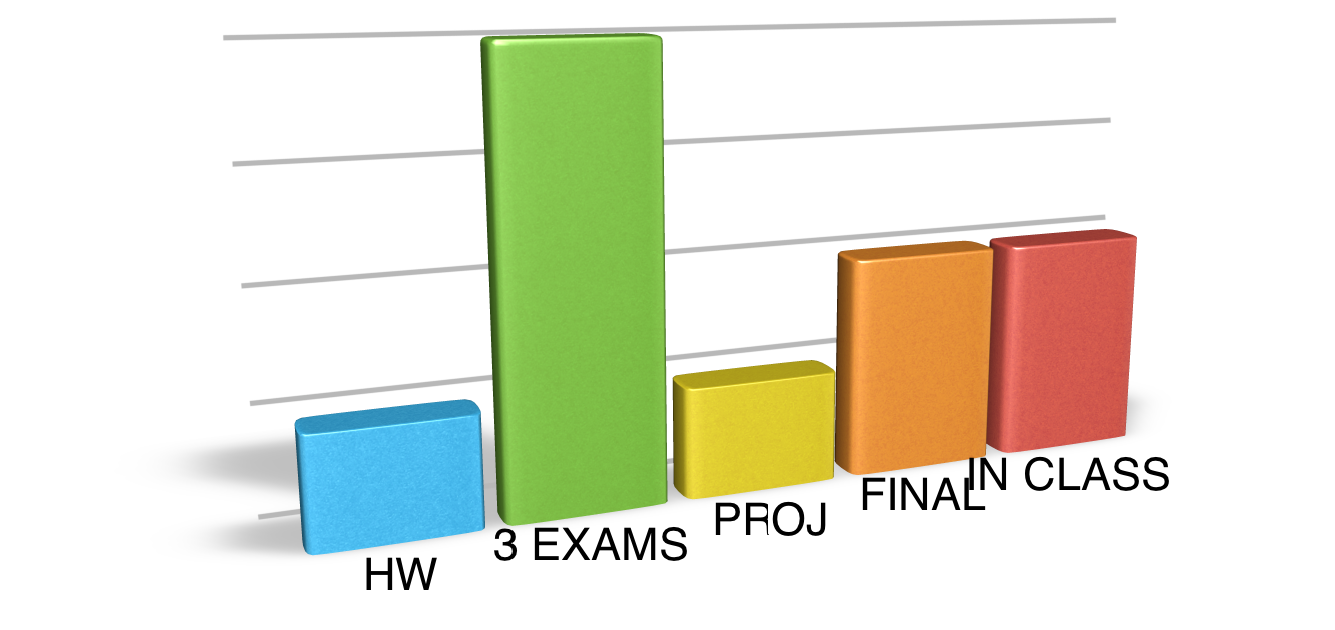
\includegraphics[width=\textwidth]{barchart.png}
    \end{minipage} \hfill
    \begin{minipage}{0.45\textwidth}
      \begin{tikzpicture}
        \pic{piechart};
      \end{tikzpicture}
    \end{minipage}
  \end{figure*}
\item Put a star next to the chart whose legend looks accurate. For each of the other charts, write down at least one reason why the legend does not make sense.

  \begin{figure*}[h!]
    \centering
    \begin{minipage}{0.45\textwidth}
      \begin{tikzpicture}
        \pic{piechart};
        \foreach \w/\x/\y/\z in {1.8/cba/Exams/50\%, 1.3/cbb/Project/15\%, 0.8/cbc/In class/10\%, 0.3/cbd/HW/20\%, -0.2/cbe/Final/25\%}
        {
          \draw[fill=\x] (3.2,\w) circle [radius=0.1];
          \node[anchor=east] at (3.1,\w) {\z};
          \node[anchor=west] at (3.3,\w) {\y};
        }
      \end{tikzpicture}
    \end{minipage} \hfill
    \begin{minipage}{0.45\textwidth}
      \begin{tikzpicture}
        \pic{piechart};
        \foreach \w/\x/\y/\z in {1.8/cba/Exams/40\%, 1.3/cbb/Project/15\%, 0.8/cbc/In class/15\%, 0.3/cbd/HW/10\%, -0.2/cbe/Final/20\%}
        {
          \draw[fill=\x] (3.2,\w) circle [radius=0.1];
          \node[anchor=east] at (3.1,\w) {\z};
          \node[anchor=west] at (3.3,\w) {\y};
        }
      \end{tikzpicture}
    \end{minipage}

    \begin{minipage}{0.45\textwidth}
      \begin{tikzpicture}
        \pic{piechart};
        \foreach \w/\x/\y/\z in {1.8/cba/Exams/40\%, 1.3/cbb/Project/10\%, 0.8/cbc/In class/10\%, 0.3/cbd/HW/30\%, -0.2/cbe/Final/10\%}
        {
          \draw[fill=\x] (3.2,\w) circle [radius=0.1];
          \node[anchor=east] at (3.1,\w) {\z};
          \node[anchor=west] at (3.3,\w) {\y};
        }
      \end{tikzpicture}
    \end{minipage} \hfill
    \begin{minipage}{0.45\textwidth}
      \begin{tikzpicture}
        \pic{piechart};
        \foreach \w/\x/\y/\z in {1.8/cba/Exams/40\%, 1.3/cbb/Project/10\%, 0.8/cbc/In class/25\%, 0.3/cbd/HW/15\%, -0.2/cbe/Final/10\%}
        {
          \draw[fill=\x] (3.2,\w) circle [radius=0.1];
          \node[anchor=east] at (3.1,\w) {\z};
          \node[anchor=west] at (3.3,\w) {\y};
        }
      \end{tikzpicture}
    \end{minipage}
  \end{figure*}
  
\item Using the chart that you marked accurate from exercise 3, fill in the weight of each
  category using fractions. Write fractions in lowest terms.

  \begin{figure*}[h!]
    \centering
    \begin{tikzpicture}
      \pic{piechart};
      \foreach \w/\x/\y/\z in {1.8/cba/Exams/40\%, 1.3/cbb/Project/10\%, 0.8/cbc/In class/25\%, 0.3/cbd/HW/15\%, -0.2/cbe/Final/10\%}
        {
          \draw[fill=\x] (3.2,\w) circle [radius=0.1];
          \node[anchor=west] at (3.3,\w) {\y};
        }
    \end{tikzpicture}
  \end{figure*}

  \clearpage
\item If you were teaching this class, how would your pie chart look on your syllabus? Don’t
  worry about attaching numbers, just represent your idea graphically.

  \begin{figure*}[h!]
    \centering
    \begin{tikzpicture}
      \draw (0,0) circle [radius=2cm];
    \end{tikzpicture}
  \end{figure*}
\item Will an understanding of the pie chart change how you manage your study time for this
class? Explain your answer.
\end{enumerate}

\end{document}

%%% Local Variables:
%%% mode: latex
%%% TeX-master: t
%%% End:
